%%% -*-LaTeX-*-
\chapter{Drawing Lessons from Modern NICs}
\label{chap:modernnics}
Network Interface Cards have grown complex and present opportunities and challenges as part of a modern distributed system.
 It is imperative that today’s database system designer considers the network in design decisions.
 Previous research for optimising databases were focussed more on processing time spent on a database query~\cite{dbmsproctime},
  but today, most of the end-to-end latency while processing a query is spent the networking stack~\cite{ramcloudosr}.
Since in-memory databases became popular and datasets started to fit in memory, the spinning disks 
which were the primary I/O bottlenecks before aren't anymore. The bulk of I/O overhead in a distributed storage system today is in network transmission.
Adding this to the fact that the modern NIC allows us to offload CPU from the data transfer path,
the saved memory bandwidth and CPU cycles could be doing useful work.

Hardware overheads have thinned over time, and system researchers had to minimize CPU interrupts and come up with forms of kernel by-pass networking to extract more performance.
 Network cards have had Transmission Control Protocol(TCP) offloading baked in as TCP Offload Engine for some time now. They helped reduce TCP protocol burden from main CPU by moving that processing to network adapters.
 However the ability to bypass copies were dependent on the TCP Offload Engine(TOE) design and in may cases didn't support non-copying for incoming data streams~\cite{tcpoffload}. 
 RDMA~\cite{rdmapatent,rdmacase,rdma} capable NICs support non-copying of incoming data streams over a wider variety of applications where TCP offloading was just one among the benefits involved.
 Development of advanced host-device interconnects such as PCI Express~\cite{pcie}  made it possible to develop highly performant network devices offering throughputs and latencies orders of magnitude better than what was possible before.

 The key consideration we explore in this chapter is how a database server can make the best use of the NIC’s ability to receive and transmit data directly at the application level, especially for the
cases when the system must move large chunks of data. We evaluated
the use of various RDMA primitives for benchmarking large transfers and explored the various
 trade-offs and design choices while using advanced NIC features and drew lessons from our evaluation of those choices with the help of a microbenchmark. 

\section{Zero Copy and Copy Out}
The key benefit of a modern NIC in contrast with earlier hardware is the ability to manipulate control structures of the NIC from userspace applications. 
Kernel bypass is a ubiquitous feature in the modern NIC that avoids CPU in the data transfer path. Literature defines kernel-bypass as communication that doesn't 
involve kernel in the critical path~\cite{unetkernelbypass}. Newer network controllers also make use of vectored I/O, otherwise known as scatter/gather I/O
where the NIC can receive and transmit directly from application vectors. The Mellanox Infiniband ConnectX\textregistered-3
NIC that we profiled can collect scattered chunks of data in memory via Direct Memory Access(DMA).

Before kernel bypass became commonplace, the steps for copying data over the network using socket programming 
required the host CPU to make additional copies of transmitted data.
The application calls a send function in a socket library and the data for sending is assembled 
in a transmit buffer, this transmit buffer is copied on to the on-NIC buffers, and the data is 
sent over the wire. We could employ the same technique in the kernel bypass capable NIC as well.
If we exploit the scatter/gather list to transmit data directly from where they live in memory, 
we could reduce the number of times data is copied within the host before transmission. 
This style of transmitting data which minimises the number of copies is what we'll refer as \enquote{\textbf{Zero Copy}} from now on.
Instead of employing a multi-entry scatter/gather list, the data to be transmitted, which could be discontiguous in memory, could be assembled 
onto a temporary buffer and this buffer could be treated as a single entry scatter/gather list
and then transmitted over the network. We will be calling this technique \enquote{\textbf{Copy Out}} for the remainder of the thesis. 


Zero copy DMA facilitates a scatter gather list of buffer descriptors
which could be mapped to discontiguous locations in memory on demand. These provide
the added benefit that network headers do not need to exist along with data and help bring more flexibility 
in deciding the transport layer. One subtle thing to note here is that Zero Copy only implies the absence 
of a copy of the records to a buffer. The data still needs to be copied to the on-NIC buffers before 
it is sent out via the network cable. This approach is different from what happens when we call socket send on 
a traditional stack where the data for transmission is pre-assembled in a large buffer in main memory 
and then copied across the network. We evaluate how Zero Copy performs in contrast 
with the more traditional Copy Out from now on.

\section{Memory Bandwidth}
Interestingly, the additional copy involved in Copy Out hurts memory bandwidth of the system more than contributing 
to additional CPU load purely from the perspective of network transmission. Our evaluation in Section~\ref{sec:overhead} shows us that while the traditional
copy adds only up to 18\% increase in overhead of total CPU utilization, the effect on memory bandwidth is worse.
 If we were to make use of the high throughput available in NICs by transmitting near line rate using Copy Out, 
 the transmission takes up 2$\times$ more memory bandwidth which accounts for half of the total available memory bandwidth in a modern server.
  We should read this in the context that network transmission is not the primary responsibility of a storage server in a distributed system
   and costs of communication should be treated as overhead. Most of the memory bandwidth is wasted in just aggregating the data 
before transmission could be used as part of actual computation or other useful rearrangements of data in 
the query response. Section~\ref{sec:impact} will fully discuss the impact on memory bandwidth and other parameters while the system 
is transmitting large amounts of data.


\section{NIC structures in detail}
Figure~\ref{fig:mem-regions} details how an application interacts with a Mellanox
ConnectX-3\textregistered , a modern 56~Gbps NIC that uses kernel bypass. 
With Zero Copy, transmit descriptors list several chunks of data for
the NIC to DMA. With Copy Out, all data to be transmitted is first explicitly
copied into a transmit buffer by the host CPU; then, a transmit descriptor is
posted that references just the transmit buffer rather than the 
source data. Both Zero Copy and the traditional Copy Out approaches to transmission are shown.
In both cases, the same three key data structures are involved. 

The first important structure is the
data to be transmitted, which lives in heap memory. For Zero Copy, the memory
where the records live must first be registered with the NIC. Registration
informs the NIC of the virtual-to-physical mapping of the heap pages. This is
required because the NIC must perform virtual-to-physical address translation
since the OS is not involved during transmission and the application has no
access to its page tables. Registration is done when the beginning of the benchmark and is often
done with physical memory backed by 1~GB hugepages to minimize on-NIC address
translation costs.
\begin{figure}[t]
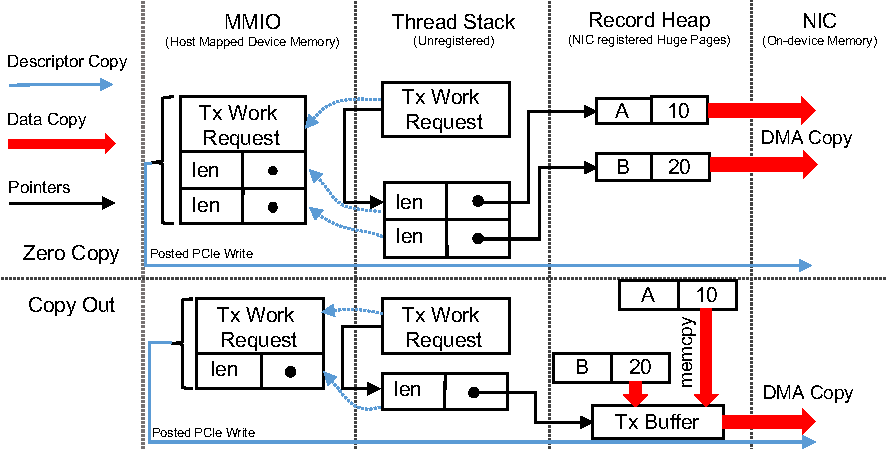
\includegraphics[width=\textwidth]{fig-mem-regions.pdf}
\caption{Key structures involved in network transmission.}
\label{fig:mem-regions}
\end{figure}



The second key structure is the descriptor that a thread must construct to
issue a transmission. With Mellanox NICs, a thread creates a work request and a
gather list on its stack. The work request indicates that the requested
operation is a transmission, and the gather list is a contiguous list of
base-bound pairs that indicate what data should be transmitted by the NIC (and
hence DMAed). For zero-copy, the gather list is as long as the number of chunks
that the host would like to transmit, up to a small limit. The NICs we use support
posting up to 32~chunks per transmit operation. Later, we find that this small
limit bottlenecks NIC transmit performance when chunks are small and numerous.

The final important structure is the control interface between the NIC and the
host CPU.  When the NIC is initially set up by the application, a region of the
NIC's memory is mapped into the application's virtual address space. The NIC
polls this region, and the host writes new descriptors to it from the thread's
stack to issue operations. The region is mapped as write-combining; filling a
cache line in the region generates a cache line sized PCIe message to the NIC.
The NIC receives it, and it issues DMA operations to begin collecting the data
listed in the descriptor. The PCIe messages are posted writes, which means they
are asynchronous from the CPU's perspective. Even though PCIe latencies are much
higher than DRAM access, the CPU does not stall when posting descriptors, so the
exchange is very low overhead.

\subsection{Structural differences in Zero Copy and Copy Out}
The key difference between Zero Copy and Copy Out is shown with the wide, red
arrows in Figure~\ref{fig:mem-regions}. Copy Out works much like conventional
kernel-based networking stack: chunks of data are first copied into a single
transmit buffer in host memory, usually by a \memcpy ~call to copy from the record's 
virtual address to the transmit buffer. Then, a simple, single-entry descriptor is
posted to the NIC that DMAs the transmit buffer to an on-device buffer for transmission.
As a result, copy-out requires an extra and explicit copy of the data, which is made
by the host CPU.  Making the copy uses host CPU cycles, consumes memory
bandwidth, and is pure overhead. 
% Rob was of the opinion to cut this here since lessons should either be in chapter
% beginning or after evaluations
% Surprisingly, though, copy-out has
% advantages including better performance when
% records are small and scattered.  In those cases, complex gather descriptors
% bottleneck the NIC, and using the host CPU to pre-assemble the responses can
% improve performance.



\section{DDIO}
One conflating factor in understanding the benefits of Zero Copy is Data Direct I/O (DDIO)~\cite{ddio}.
 DDIO is a performance-oriented enhancement to the DMA mechanism which was introduced in Intel\textregistered Xeon E5 processors with Sandy Bridge-EP micro-architecture.
 With DDIO, CPU caches are used as the primary source and destination for I/O, 
allowing network interface controllers (NICs) to talk directly to the last level caches of local CPUs
and avoid costly fetching of the I/O data from system RAM. As a result, if we have enough locality of data to exploit,
DDIO reduces the overall I/O processing latency, allows processing of the I/O 
to be performed entirely in cache and prevents the available memory bandwidth from becoming a performance bottleneck.
We fully investigate the effects of DDIO in Section~\ref{sec:impact} to conclude the impact of 
Copy Out mechanism.


\section{Inlining}
Mellanox NICs allow some data to be {\em inlined} inside the control message
sent to the NIC over PCIe. Our NICs allow up to 912~B to be included in the
descriptor that is posted to the NIC control ring buffer.  Inlining can improve
messaging latency by eliminating the delay for the NIC to DMA the message data
from host DRAM, which can only happen after the NIC receives the descriptor.
Inlining benefits small request/response exchanges, but it does not help for
larger transmissions. This is because even though there is an extra delay
before the NIC receives the actual record data, that delay can be overlapped
with the DMA and transmission of other responses. Other researchers have shown
that sending data to the NIC via MMIO also wastes PCIe bandwidth~\cite{rdma}.
All of our experiments have inlining disabled. Enabling inlining gives almost 
identical throughput, and overhead, except it only works for transmissions of ~912 B or less.

\section{Eliminating Contention}
\label{sec:code-optimisation}
In our original implementation, we used a common shared buffer pool for transmission.
We later found that the use of thread local transmit buffers to avoid contention on the buffer pool during 
Copy Out transmission shows considerably less overhead due to busy waiting to get free transmit buffers 
and accentuates the effect of DDIO. This differs from the published results~\cite{imdmpaper}. 
The measurements in this thesis only include data collected after the optimisation.

\section{Evaluation}
% TODO
% Should we put the tx buffers in huge pages?
% Knowing measured peak mem bw of our machines would be good, but it looks like
%   not all channels are populated?
We wanted to show the impact of NIC features on large databases which often have to 
transmit significant amounts of data while responding to range scans or reconfiguring clusters. 
We evaluated various choices in the design space that a database designer encouters while developing 
a database that is NIC friendly. We set up the following experiments and found compelling 
evidence that will aid in co-designing databases for new hardware.
\begin{itemize}
\item Comparison of various RDMA primitives over Mellanox Infiniband verbs library; we find that \cpp{SEND} is best suited for returning scattered records.
\item Comparison of different arrangements of small 128~B records to evaluate how to best exploit S/G DMA; we find Zero Copy, {\em when carefully tuned} offers better throughput and efficency. We outline precisely when Copy Out can be faster 
and more efficient than Zero Copy which could be exploited for small gains.
\item Similar comparison on larger 1024~B records; we observe Zero Copy is a clear winner in terms of throughput and efficiency across the board.
\item Comparison of CPU cycles spent per transmitted byte; overheads at transmissions $<$384~B makes Copy Out more efficient while Zero Copy is a clear winner for larger transmissions and larger records.
\item A breakdown of CPU overhead in transmission; we see that the additional \memcpy ~dominates CPU overheads to the tune of 95~\%, transmission overhead for smaller transmissions are conspicous.
\end{itemize}



\subsection{Experiment Setup}
We explored hows the different designs trade-off database server efficiency and
performance by building a simple model of an in-memory database system that
concentrates on data transfer rather than full query processing. In all experiments,
one node acts as a server and transmits results to 15 client nodes.
Our experiments were run on the Apt~\cite{Ricci+:OSR15} cluster of the
CloudLab~\cite{Cloudlab:URL} testbed: this testbed provides exclusive bare-metal
access to a large number of machines with RDMA-capable Infiniband NICs.
Table~\ref{tbl:config} shows the Experiment Setup for the cluster where we profiled
the Mellanox Infiniband ConnectX-3 \textregistered NIC and impact of data layout and 
use of no update in place structures on transmission throughput. The cluster has 7
Mellanox SX6036G FDR switches arranged in two layers. The switching fabric is
oversubscribed and provides about 16~Gbps of bisection bandwidth per node
when congested. All of our experiments are publicly available online\footnote{\url{https://github.com/utah-scs/ibv-bench}}.
Figure~\ref{fig:setup} shows the experiment setup. Each of the server threads transmit to one of the 15 clients from our 16 core machine. 
Thread affinity gives better performance and accurate score boarding of performance.


All our experiments transmit from a large region of memory backed by 4~KB pages
that contain all of the records. The region is also
registered with the NIC, which has to do virtual-to-physical address
translation to DMA records for transmission.
Others have argued that in some cases, using 1~GB hugepages reduces translation lookaside buffer
(TLB) misses~\cite{infinibandhugepages}. We have realized that the NIC can benefit from
hugepages as well, since large page tables can result in additional
DMA operations to host memory during address translation~\cite{farm,rdma}. For
our experiments, the reach of the NIC's virtual-to-physical mapping is
sufficient, and hugepages have no impact on the results. To err on the side of caution, 
we did enable 1~GB hugepages and registered those with the NIC to make sure we 
avoid as many TLB misses as possible.
\begin{table}[H]
\def\arraystretch{1.25}%  1 is the default, change whatever you need
\begin{tabular}{@{}l@{\hskip 12pt}l@{}}
\toprule
\textbf{CPU} & Intel Xeon E5-2450 (2.1~GHz, 2.9~GHz Turbo) \\
    & 8 cores, 2 hardware threads each \\
\textbf{RAM} & 16~GB DDR3 at 1600~MHz \\
\textbf{Network} & Mellanox MX354A ConnectX-3 Infiniband HCA (56 Gbps Full Duplex) \\
        & Connected via PCIExpress 3.0 x8 (63~Gbps Full Duplex) \\
%        & 7 Mellanox SX6036G FDR Switches \\
\textbf{Software} & CentOS 6.6, Linux 2.6.32, gcc 4.9.2, libibverbs 1.1.8, mlx4 1.0.6 \\
\bottomrule
\end{tabular}
\vspace{0.25eX}
\caption{Experimental cluster configuration.}
\label{tbl:config}
\end{table}

\begin{figure}[H]
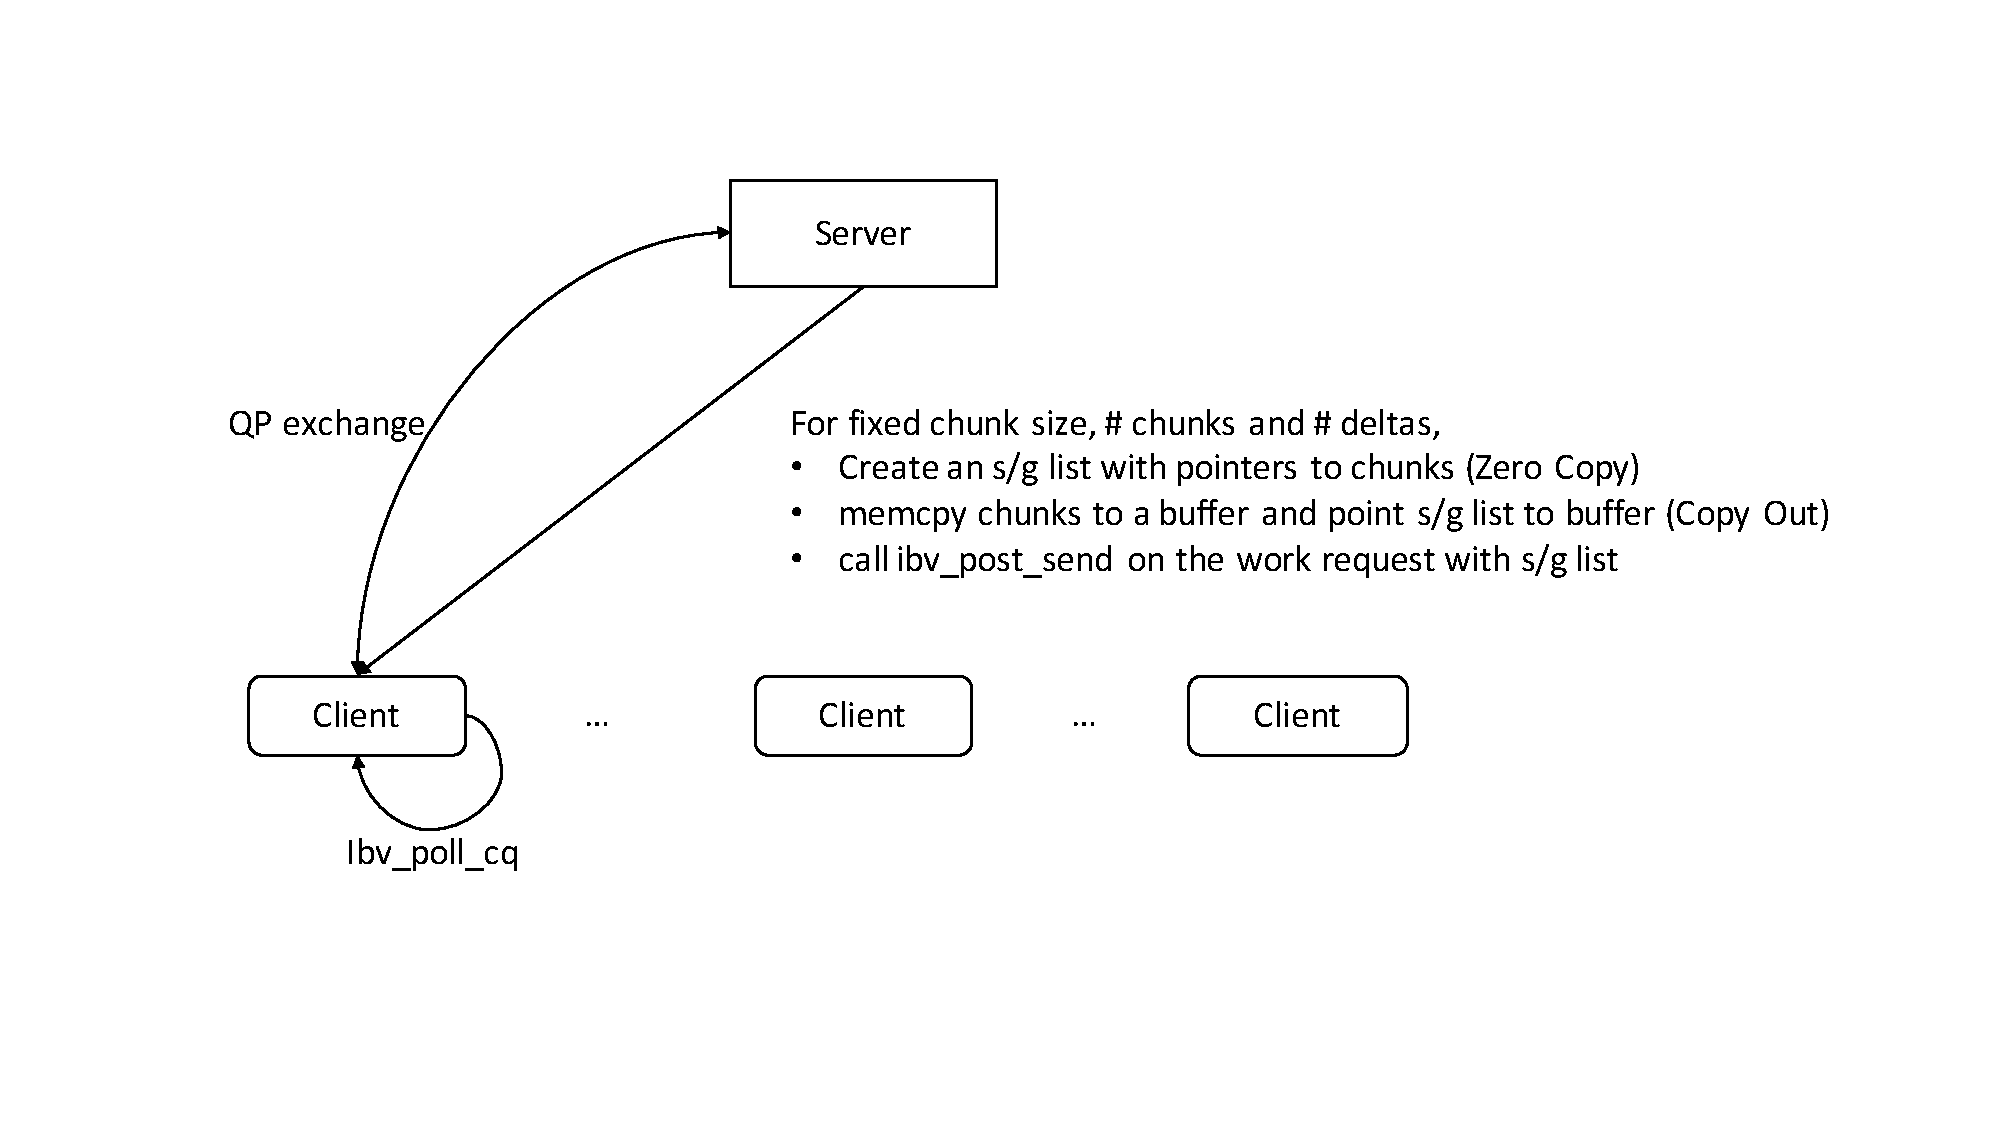
\includegraphics[width=\textwidth]{fig-setup.pdf}
\caption{Experiment setup. Each of the 15 clients communicate to a pinned thread on the server}
\label{fig:setup}
\end{figure}


\subsection{Comparing RDMA modes for transmission}
We started out by getting measurements of transmission speeds using RDMA verbs.  
READ and WRITE are the most commonly employed RDMA verbs because they are one sided
and does not require both ends to be active in theory. RDMA read has the additional incentive 
that it is client initiated. SEND/RECEIVE primitives, on the other hand, are two-sided and 
server initiated.  We evaluated the performance of each of this using Infiniband verbs library. We implemented 
RDMA reads and write as op codes on the \cpp{ibv_send_wr} request which 
transmit data via \cpp{ibv_post_send} and measured the transmit 
performance while enabling Zero Copy using \cpp{IBV_WR_SEND} as the opcode.
\cpp{SEND} operations can transmit multiple entries in the S/G list.
One issue we uncovered was that one-sided RDMA verbs are not well positioned to 
take advantage of the Zero Copy paradigm since it only supports a remote read 
from a registered location from the other side. READ also requires a secondary notification mechanism 
to work in practice negating the advantage of being one sided.
Others have argued for the use of one-sided RDMA for key-value stores~\cite{pilaf} and even for accelerating 
range queries~\cite{zerocopyrangequery}. We estimate that these would be suitable for large transmissions only when there is a strong 
correlation of queries with resulting values that are contigous in memory. In the general case, the receiver 
needs to be active and you can only gather one remote location in one call to the \cpp{ibv_post_send}.
It could work better if we were to pipeline multiple requests, but we are losing out on efficiency per operation.

Figure~\ref{fig:200B_transrate} shows a comparison of transmission
performance of different verbs transmitting 200 Bytes(B) records varying the number of records
that could be transmitted at a time for various operations. The green dot shows
the performance for RDMA READ which is also unfair since RDMA READ can only transmit from a single remote virtual address at a time.
The blue dot shows RDMA write performance using a full scatter/gather list. This tells us that WRITE and SEND will offer 
similar performance. Transmission using larger data sizes such as 1000~B recoreds showed a clearer benefit of using \cpp{SEND} than 
using 200~B records as shown in Figure~\ref{fig:1000B_transrate}.
\begin{figure}[H]
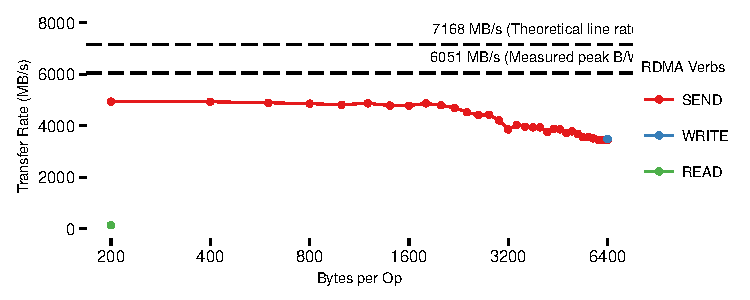
\includegraphics[width=\textwidth]{fig-200B-RDMAverbs}
\caption{Transmission rate for 200 B records over different RDMA verbs and 
varying S/G lengths. We only show \cpp{WRITE} at full capacity and \cpp{READ} at one read per transmission.}
\label{fig:200B_transrate}
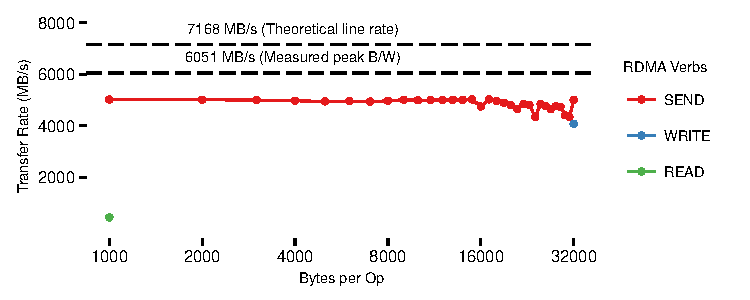
\includegraphics[width=\textwidth]{fig-1000B-RDMAverbs}
\caption{Transmission rate for 1000 B records over different RDMA verbs and 
varying S/G lengths. We only show \cpp{WRITE} at full capacity and \cpp{READ} at one read per transmission.}
\label{fig:1000B_transrate}
\end{figure}


\framebox[0.9\textwidth][c]{
  \parbox{0.7\textwidth}{
\cpp{SEND} saturates NIC; Can gather records and notify receiver when transmission completess
\par
 \cpp{WRITE} avoids invoking receiver; Server should induce notifications some other way.
 \par
 \cpp{READ} is client initiated; It's the lowest overhead on server, but can only collect one contigous chunk per posted op limiting it's usefulness for returning complex responses.}
}
\captionof{Takeaway}{ Use \cpp{SEND} RDMA verbs for returning scattered set of records \label{takeaway:verbs}}


\subsection{Record Sizes}
In the world of In-memory databases, there is an argument to be made that record sizes will get smaller.
The decreased access latency of in-memory databases makes them well-suited to smaller, finer-grained records
than were previously common. One expectation is that this will drive databases
toward more aggressively normalized layouts with small records. This
seems to be increasingly the case as records of a few hundreds bytes or less
are now typical even for companies that manage large volumes of data in memory~\cite{fb-memcache,fb-workload,inmemoryworkload}. 
We choose 128~B records as a realistic sample of record sizes in the future and compare it against 
1024~B records to see the performance impact due to bounded-disorder in our evaluations in the rest of the thesis.



\subsection{Performance Impact of Data Layout}
\label{sec:zero-copy-tput}

% stutsman: some old dead text, probably totally worthless.
% At some point make sure the rest of the text contains all of these ideas
% already.
%
% Smaller transmissions require more NIC interaction and PCI Express (PCIe)
% writes to transmit query results, but they can deal with discontinuous
% in-memory data layouts. In the case of zero-copy transmission, smaller
% transmissions may also reduce the amount of time that the database must keep
% records stable for the NIC.  Larger transmissions can also accommodate
% discontinuity through two different methods: copy-out or zero-copy, but
% discontinuity results in increased transmit descriptor size and complexity.
To explore how different design decisions affect trade-offs in server efficiency and
performance, we built a simple model of an in-memory database system that
concentrates on data transfer rather than full query processing.

The first key question is understanding how database record layout affects the
performance of the transmission of query results.  The transmission of large
result sets presents many complex choices that affect
database layout and design as well as NIC parameters.  Range query
results can be transmitted in small batches or large batches and either via
Copy Out or Zero Copy.

To understand these trade-offs, we measure the aggregate transmission
throughput of a server to its 15~clients under several
configurations.  In each experiment, the record size, $s$, is set as either 1024~B or
128~B. Given a set of records that must be transmitted, they are then grouped
for transmission. For zero-copy, an $n$ entry DMA gather descriptor is created
to transmit those records where $ns$ bytes are transmitted per NIC transmit
operation. For copy-out, each of the $n$ records is copied into a single
transmit buffer that is associated with a transmit descriptor that only points
to the single transmit buffer. Each transmission still sends exactly $ns$
bytes, but copy-out first requires $ns$ bytes to be copied into the transmit buffer.
We vary $n$ from 1 to as much as the NIC can support DMAing in a single transmission.
Intuitively, larger groups of records (larger sends) result in less host-to-NIC
interaction, which reduces host load and can increase throughput; the actual benefits
depend on the specific configuration and are explored below.

Figure~\ref{fig:zero-copy-tput} shows how each of these configurations impacts
transmission throughput. For larger 1024~B records, using the NIC's DMA engine
for Zero Copy shows clear benefits even when you are transmitting less number of 
records. This is in addition to the CPU and memory bandwidth savings, which 
we explore in Section~\ref{sec:overhead}). The database server can 
saturate the network with Zero Copy as long as it can post 2 or more
records per transmit operation to the NIC (that is, if it sends 2~KB or larger
messages at a time). For the Copy Out approach, you get roughly the same transmission 
throughput as Zero Copy when your transmission sizes get bigger at around 16~KB. In 
the impact study in Section~\ref{sec:impact} we explain why this is not a good value 
proposition. We saw the DMA engine could provide a throughput boost
of up to 86\% over Copy Out while transmitting two 1024~B records. It's also interesting 
to note that if range scans return even just 16 scattered, small(128~B) records per query, the
benefits of Zero Copy purely from the perspective of transmission throughput is almost eliminated.
\begin{figure}[t]
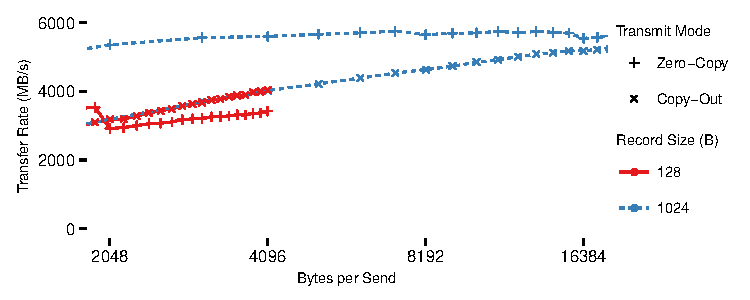
\includegraphics{fig-zero-copy-tput.pdf}
\caption{Transmission throughput for Zero Copy and Copy Out.}
\label{fig:zero-copy-tput}
\end{figure}


% computePctTputImprovementForZeroCopy(loadMerged())
% [1] "128 B item pct improvement in tput for zero-copy"
%  [1]   8.105552  10.928705  14.097586  18.910805  28.721654  43.346138  51.993156  44.439383  55.446378
% [10]  43.414034  35.736397  26.654478  23.842016  20.787579  18.376618  -5.310453  -2.382863  -4.469114
% [19]  -5.565349  -6.927329  -6.270677  -7.919818  -8.681226  -9.356702 -11.269678 -11.943183 -12.265026
% [28] -13.209408 -13.396745 -13.930867 -14.057826 -12.286999
% [1] "Max 55.4463782269341"
% [1] "1024 B item pct improvement in tput for zero-copy"
%  [1] 53.841302 86.064417 55.299614 40.553317 37.989062 33.750689 30.841420 23.594658 21.917508 19.037890
% [11] 18.186771 15.621109 14.475694 12.246097 11.008283  7.318041  7.586871  7.262891  7.572221  7.396499
% [21]  7.427524  7.109614  7.039692  6.980079  6.610857  5.824279  5.979297  5.631181  5.694890  5.299445
% [31]  5.746029  5.610679
% [1] "Max 86.0644167799178"



%Copy Out 128 B - 8chunks(1024B) - 2400 MB/s
%Copy Out 128 B - max 32 chunks - 3885MB/s
%Copy out 1024B  -max 32chunks - 5507MB/s
%ZeroCopy 128 B - chunks-MB/s, 1-526,7-3430,8-3466,9-3450,10-3417,
% 11-3431,12-3375,13-3437,14-3493,15-3532,16-2908, 30-3314,31-3304,32-3408
%ZeroCopy 1024 B - 1-3841, 2-5861, 32-5816

Figure~\ref{fig:zero-copy-tput} shows that for small 128~B records, Zero Copy
provides little throughput benefit if you were only returning a few records 
at a time. Our NIC is limited to gather lists
of 32~entries, which is insufficient to saturate the network with such a small
record size. Transmission peaks at 3.4~GB/s. In fact, Zero Copy performs best when
we transmit between 8-15 records or 1 to 2~KB per transmission above which the transmit performance 
tapers off. Zero Copy gives around 55\% improvement over Copy Out while dealing 
with transmissions around 1~KB or 8 records. Throughput dips with 16 records per send operation and it gradually moves up as we 
increase the transmission sizes further but never gets back to the peak transmission. This calls 
for careful attention to the length of S/G list in order for a database designer to get peak performance while using small record sizes and larger 
transmissions. We dig deeper into this anomaly and find evidence as to why this happens with the 
help of measuring traffic induced in the Memory controller due to LLC misses because of DDIO and 
PCIe traffic in Section~\ref{sec:impact}. Owing to this abberation, copying 128~B records 
on-the-fly can significantly outperform Zero Copy transmission when there are 
enough results (more than 16 records in our NIC which is capable of transmitting 32 at once) to group per transmission.
In fact, Copy Out can saturate the network with small records, and it
performs similar to Zero Copy with larger 1024~B records.

\framebox[0.9\textwidth][c]{
  \parbox{0.7\textwidth}{
  \textbf{Takeaways: Throughput}
  \begin{enumerate}
  \item Bigger records can saturate the NIC;Zero Copy is significantly faster for bigger chunks.
  \item Zero Copy is limited by the length of S/G list; This limits bytes transmitted per operation for small records.
  \item Copy out can be faster for smaller records unless S/G length is carefully tuned; We examine Copy Out's efficiency in Section ~\ref{sec:overhead}
  \end{enumerate}
  \textbf{Recommendation}: For large sets of small, scattered records, use Copy Out. If your record sizes are bigger, always use Zero Copy \label{takeaway:tput}
 }}


\section{System Impact}
\label{sec:impact}

We saw how the Zero Copy promises savings enhanced performance 
in the previous section. To put things in the context of resource utilisation and
 to quantify performance gains, we profiled our benchmark code for CPU utlisation, memory bandwidth 
 and some other metrics such as memory pressure due to Last Level Cache(LLC) misses from DDIO and PCIe.
We used cycle counters present in the original RAMCloud~\cite{ramcloud} code base for non intrusive profiling 
of CPU time.
We wanted to make sure our profiling code shouldn't interfere with the timing of our highly performant 
 benchmark which churns out millions of operations per second and microsecond latencies. 
 We searchaed for light weight profiling methods which adds minimal overheads.
 We ended up using Intel\textregistered's Performance Counter Monitoring module~\cite{intelpcm}. 
 An interesting thing about measuring performance 
 of a modern CPU is that almost all of the metrics of significance exist outside of the cores. These measurements 
 are classified as uncore or offcore measurements in the Performance Monitoring Unit(PMU) moniker.
 The newer generation CPUs that we used had the Sandy Bridge microarchitecture which provide uncore performance 
 monitoring unit and we measured their performance counters to accurately gauge impact.


\subsection{Breakdown of CPU costs}
\label{sec:overhead}

While we just showed in Section~\ref{sec:zero-copy-tput} that judicious use of Zero Copy results in enhanced transmission performance
, the goal of zero-copy DMA is to also mitigate the server-side CPU cost. Figure~\ref{fig:overheads} breaks down
CPU time for all the scenarios; small and large records using Zero Copy and Copy-Out. In the case 
of Zero Copy, most of the server CPU time is spent idling waiting for the NIC 
to complete transmissions at smaller record sizes. For 128~B records,
smaller transmissions take up more fraction of CPU owing to the overhead of more descriptors
per transmission. Zero-copy always reduces the CPU load of the server in all record sizes except for the cases where
overheads for a small number of small records and, as expected, there is a bigger
benefit for larger record sizes. 
With 1024~B records, the \memcpy ~step of Copy-Out uses a maximum of 18\% of all available
CPU cycles. What's alarming is the fact that this constitues ~95\% of all the time spent busy waiting.
This is a pure overhead that we could eliminate by using Zero Copy. While Zero Copy eleminates the \memcpy ~overhead, it adds an overhead of its own to create and copy transmit descriptors.
Each gather entry adds 16~B to the descriptor that is posted to the NIC.
These entries are considerable in size compared to
small records, and they are copied twice. The gather list
is first staged on the thread's stack and passed to the userlevel NIC driver. Next,
the driver makes a posted PCIe write by copying the descriptor (including the
gather entry) into a memory-mapped device buffer.
\begin{figure}[H]
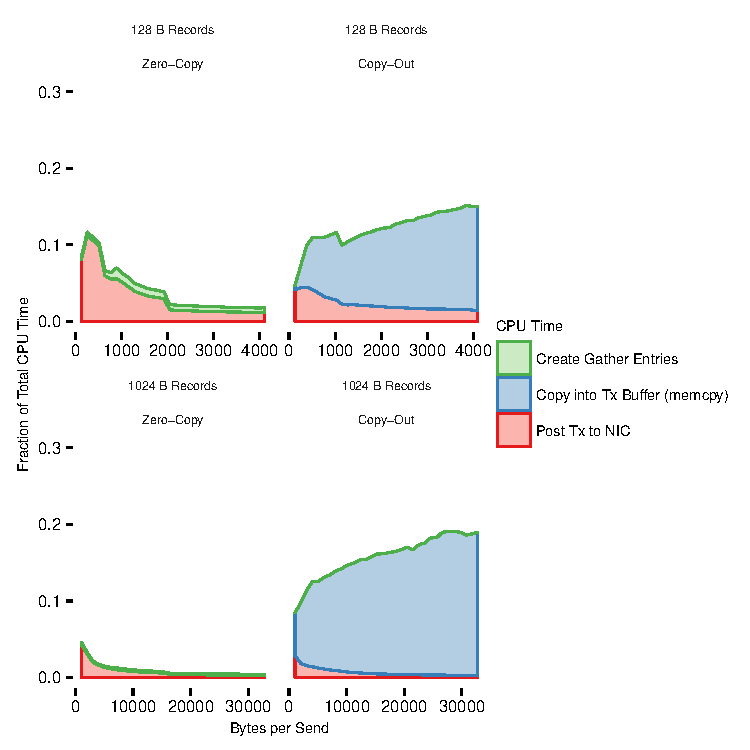
\includegraphics{fig-overheads.pdf}
\caption{Breakdown of absolute CPU overheads for transmission.}
\label{fig:overheads}
\end{figure}





We will see later in Section~\ref{sec:membw-savings} that memory bandwidth savings for zero-copy are more substantial.
Figure~\ref{fig:zero-copy-tput} shows that copy-out transmit performance nearly
matches zero-copy (5.6~GB/s versus 5.8~GB/s) for larger records at larger transmissions. Copy-out introduces exactly one
extra copy of the data, and \memcpy~reads each cache line once and writes it
once. So, copy-out is expected to increase memory bandwidth consumption
by 2$\times$ the transmit rate of the NIC or 11.2~GB/s in the worst case.  This
accounts for about 45\% of the available memory bandwidth for the server that we used. Whether
using zero-copy or copy-out, the NIC must copy data from main memory, across the PCIe bus, to its own buffers, which
could end up using another 6~GB/s of memory bandwidth. With these estimates in mind, we extensively profiled
 our benchmark with Intel's PMU module and the details of that is given in Section~\ref{sec:membw-savings}.

\framebox[0.9\textwidth][c]{
  \parbox{0.7\textwidth}{
  \textbf{Takeaways: Breakdown of absolute CPU costs}
  \begin{enumerate}
  \item \memcpy ~dominates the CPU overheads in transmission; Zero Copy offers 8x savings for small records and 45x savings for larger records.
  \item Considerable CPU overhead means Copy Out is better at transmitting $<$384~B of data; For smaller records, overhead of adding and copying descriptors can't be ignored.
  \end{enumerate}
  \textbf{Recommendation}: If CPU overhead is the likely concern, use Zero Copy; adding an exception for this rule for transmissions $<$384~B might help minimising overheads. \label{takeaway:cpu-overhead}
 }}



% Need to know how much memory bw \memcpy/  actually burns.
% Based on pcm-memory.x and the membench tool I stuff in the ibv-bench
% directory \memcpy/  does one read and one write for each cache line it copies,
% probably at least when the copies are larger enough.
% Based on Erik's work it looks like row-buffers are 8 KB! Wow, this might
% actually impact our story in terms of energy efficiency!

% computeBestCyclesPerRecordImprovement(loadMerged())
% [1] "1773889090.13867 624551729.013333 2961703308.21867 148009809.173333"
% [1] "Pct overhead reduction of nocp versus cp for"
% [1] "128 B records"
% [1] 64.79195
% [1] "1024 B records"
% [1] 95.00254
% > 

\subsection {CPU Efficiency of transmission}
The results from previous section break down where the CPU savings come from,
but not all configurations result in the same transmit performance. For
example, Figure~\ref{fig:zero-copy-tput} shows that when transmitting
128~B~records, copy-out gets up to 15\% better throughput than zero-copy while transmitting
32~records at once. As a result, minimizing CPU overhead can come at the expense of transmit
performance. CPU overheads as a total fraction of CPU tells us what makes up for the overheads 
in transmission where CPU cost per transmitted byte will tell us the CPU efficiency of the 
transmission. The real CPU efficiency of the server in transmission is shown in
Figure~\ref{fig:cycles}. The figure shows how many cycles of work the CPU needs to do
for every byte transmitted in each of the configurations, which reveals two key things.
First, it shows that, though the absolute savings in total CPU cycles is small
for zero-copy, it does reduce CPU overhead due to transmission by up to 95\% for 
larger records and around 64\% for smaller records. For smaller records, small transmission
results in more CPU usage (till around 3~records or 384~B) owing to the overhead of descriptors.
\begin{figure}[H]
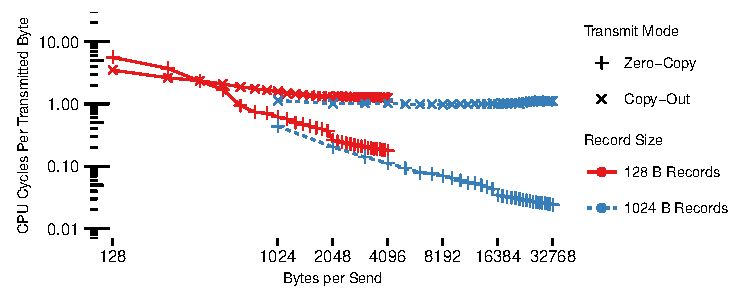
\includegraphics{fig-cycles.pdf}
\caption{Cycles per transmitted byte for large and small records with zero-copy and copy-out. Note the log-scale axes.}
\label{fig:cycles}
\end{figure}



\framebox[0.9\textwidth][c]{
  \parbox{0.7\textwidth}{
  \textbf{Takeaways: CPU Efficiency of Transmission}
  \begin{enumerate}
  \item Most efficient CPU utilization for transmission is obtained while using Zero Copy on large batches; 72\% savings for 128~B records and 95\% savings for 1024 B records
  \item Zero Copy is 2x costlier than Copy Out in transmitting a single 128B record; results like equality searches on small records might be better served by Copy Out.
  \item If the results to be transmitted involve 2 or more records, Zero Copy is always more CPU efficient.
  \end{enumerate}
  \textbf{Recommendation}: Zero Copy effectively offloads CPU and cost per byte goes down drastically when you transmit larger batches of records \label{takeaway:cpu-cycles}
 }}


% LMBench 3.0 Memory Results from our Machines
% *Local* Communication bandwidths in MB/s - bigger is better
% -----------------------------------------------------------------------------
%  Host                OS  Pipe AF    TCP  File   Mmap  Bcopy  Bcopy  Mem   Mem
%                               UNIX      reread reread (libc) (hand) read write
% --------- ------------- ---- ---- ---- ------ ------ ------ ------ ---- -----
% node-0.st Linux 2.6.32-                              4813.3 5606.8 8349 6797.
%

% Copy 512 MB between two regions of a single hugepage 100 times.
% One process at a time:
% [stutsman@node-0 ~]$ ./membench
% CPU Secs 12.023564
% bw 4.158501 GB/cpuS
%
% 8 processes at a time:
% [stutsman@node-0 ~]$ CPU Secs 49.799340
% bw 1.004029 GB/cpuS
% CPU Secs 49.842697
% bw 1.003156 GB/cpuS
% CPU Secs 49.905588
% bw 1.001892 GB/cpuS
% CPU Secs 50.420696
% bw 0.991656 GB/cpuS
% CPU Secs 50.585852
% bw 0.988419 GB/cpuS
% CPU Secs 50.699039
% bw 0.986212 GB/cpuS
% CPU Secs 50.757823
% bw 0.985070 GB/cpuS
% CPU Secs 50.850676
% bw 0.983271 GB/cpuS

% > sum(d[d$chunkSize == 128 & d$chunksPerMessage == 64,]$mbs)
% [1] 4438.671



\subsection{Memory Bandwidth}
In a modern In-Memory Database server, DRAM utilisation is the most precious resource~\cite{ramcloudfast}. 
 Available memory bandwidth is also at a premium since there is a direct correlation between Memory Bandwidth
 utilisation and DRAM latencies and starvation. Since uncore events will give the most accurate measurements,
 we explored all uncore events that induce pressure on the memory controller. We found that 
\texttt{LLC\_MISSES X 64} (cache line size) is an interesting metric, but there was a problem that it wouldn't account for prefetch 
 misses. We went for the more accurate \texttt{MEMORY\_BW\_READS} and \texttt{MEMORY\_BW\_WRITES} metrics which are derived from 
 \texttt{CAS\_COUNT.RD} and \texttt{CAS\_COUNT.WR} metrics which are the number of cache lines read and written in the sampling 
 interval. We used an interactive reporting tool written on top of perf with named mappings for these events
 to measure this metric. We profiled the total memory bandwidth consumed by the system while our benchmark 
 was running with fixed record sizes, number of records and mode of copying (Zero Copy and Copy Out). We took the median of our measurements 
 to account for consumption only while the system was transmitting data.


Figure ~\ref{fig:membw} shows the memory bandwidth consumed by the system while transmitting data at various modes 
of copying varying record sizes and transmission sizes. We can see that using Zero Copy on larger transmissions involving 
larger record sizes is beneficial. The savings are highlighted along largest transmissions of 32 records of sizes 1~KB each. 
 We had measured that a userspace application could achieve a peak bandwidth of around 24~GB/s in our system. This would mean that Copy out 
 might take up a half of all available bandwidth in order to saturate the NIC while transmitting. This should raise alarms for a database 
 designer since this is a pure overhead and the wasted memory bandwidth could be used for data manipulation or other useful work in the database 
 server. This is even more interesting considering that the modern day In-memory stores are not tuned for large responses.
  When the DRAM latency and accesses go up, the performance of the whole system could degrade to the point at which the system might become unusable.
\begin{figure}[t]
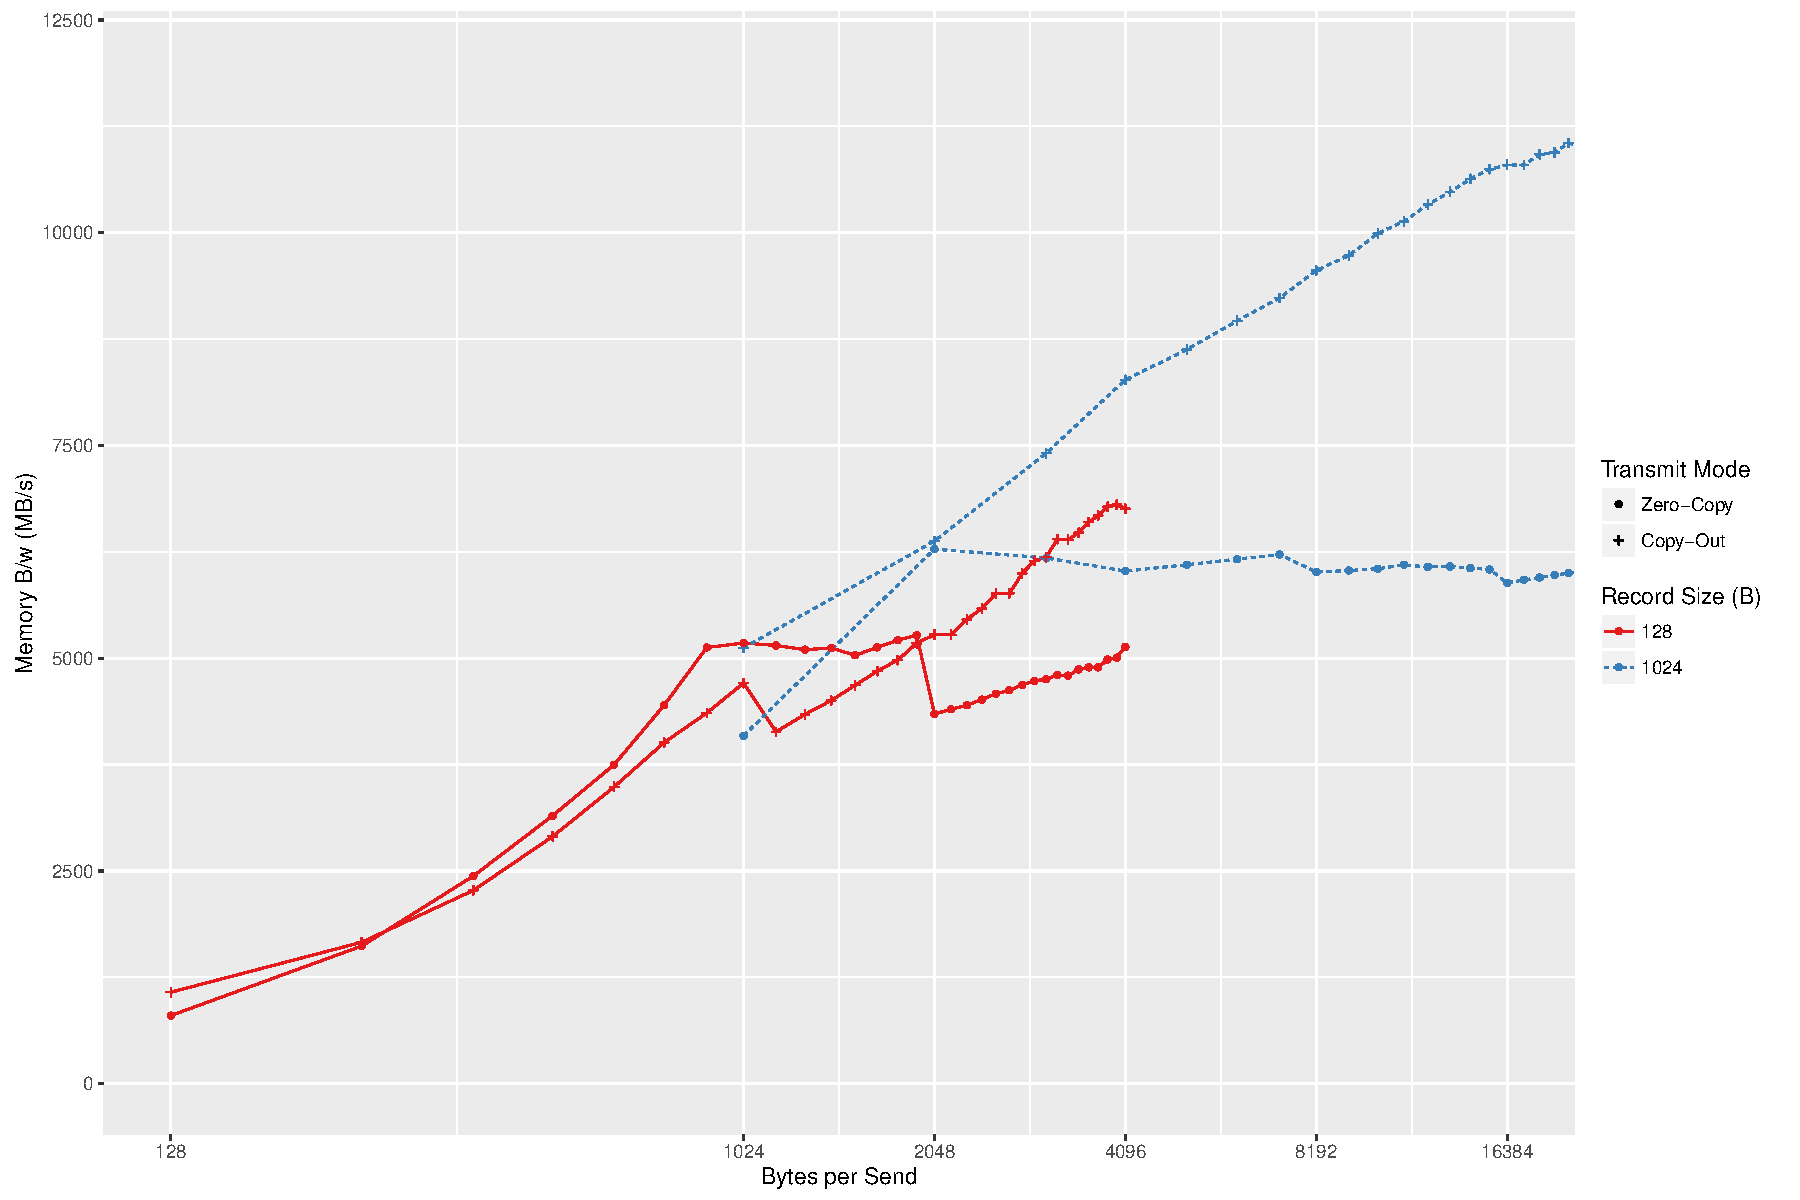
\includegraphics[width=\textwidth]{fig-membw.pdf}
\caption{Measured memory bandwidth impact on the system during transmission.}
\label{fig:membw}
\end{figure}


For smaller data sizes, it's even more interesting. Zero Copy doesn't show a huge contrast in memory bandwidth utilisation. There are times 
when Copy out outperforms Zero Copy even in terms of memory bandwidth utilisation. Its interesting to note that these data points overlap the anomalous transmit performance 
degradation we saw while observing transmission throughput in Figure~\ref{fig:zero-copy-tput}. Interestingly, after this region in the graph 
where you transmit 16 or more 128~B records where Zero Copy offers better transmission throughput, the memory bandwidth consumption by Zero Copy 
is reduced and Copy-out starts to appear more expensive in terms of memory bandwidth. These anomalies are better explained in Section~\ref{sec:anomaly} but we 
can conclude from this figure that there is a linear correlation between transmit performance and consumed memory bandwidth for Zero Copy.


\framebox[0.9\textwidth][c]{
  \parbox{0.7\textwidth}{
  \textbf{Takeaways: Impact of Memory Bandwidth}
  \begin{enumerate}
  \item Copy Out might occupy significant portion of available Memory Bandwidth; Transmissions of 32 records of 1~KB size consumed \textbf{half of all available bandwidth}.
  \item Smaller records have a smaller memory footprint and may not affect available bandwidth; The trend follows transmission throughput and there are areas where Zero Copy is costlier
  \end{enumerate}
  \textbf{Recommendation}: Zero Copying larger records saves the most memory bandwidth while giving stellar throughput. \label{takeaway:impact-membw}
 }}


\subsection{Memory Bandwidth and Transmission throughput}
\label{sec:membw-savings}
Figure~\ref{fig:membw-ratio} shows the ratio of Memory pressure exerted per bytes transmitted. We can clearly see the value proposition of 
Zero Copy mode of transmitting here. For Zero Copy, We can see that the system is consistent and predictable and only incurs a tiny overhead of 
copying descriptors other than DMAing the data on to the NIC. The overhead of the descriptors is evident from the fact that 128~B records show 
a bigger multiplier on transmission throughput than 1024~B records. For 128~B records, the ratio appears tumultous across varying number of records, 
 but still shows Zero Copy as the clear winner. If we were to compare larger 1~KB records across the two modes of copying, we can see that there is a 
 2X memory bandwidth cost on copying out 1024~B records. 
\begin{figure}[t]
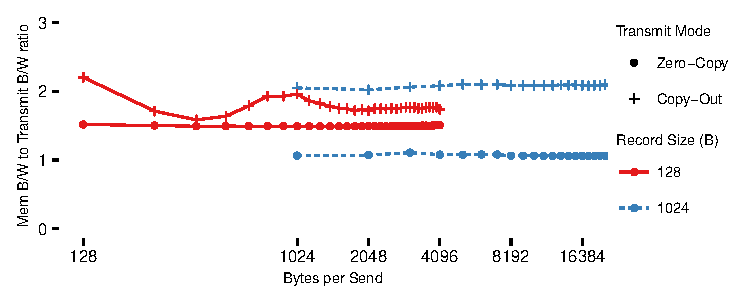
\includegraphics[width=\textwidth]{fig-membw-ratio.pdf}
\caption{Ratio of Memory Bandwidth to Transmission Throughput}
\label{fig:membw-ratio}
\end{figure}



\framebox[0.9\textwidth][c]{
  \parbox{0.7\textwidth}{
  \textbf{Takeaways: Efficiency of Memory Bandwidth Utilization}
  \begin{enumerate}
  \item Any use of Copy Out is pure overhead; Smaller records doing Zero Copy have larger memory footprint owing to the descriptor overhead
  \item There are cases where Zero Copy and Copy Out show similar memory bandwidth efficiency of transmission; Copy Out of smaller records have bigger footprint though inconsistent across transmission sizes.
  \item Chapter~\ref{chap:applications} discuss a hybrid approach yielding better throughput without consuming as much memory bandwidth.
  \end{enumerate}
  \textbf{Recommendation}: If efficient use of memory bandwidth is a concern, always use Zero Copy.\label{takeaway:impact-membw-ratio}
 }}


\subsection{DDIO traffic}
Newer generation of Intel Processor's have a portion of their Last Level Cache dedicated for I/O. This was initially called Direct Cache Access 
and more recently named DDIO. This changes our perception of memory consumption quite a bit. Network transmission occurs at this part of the Last Level Cache 
and even the destination for a packet over the network becomes this dedicated portion of LLC. This has significant impact in the number of LLC misses the system 
has to take while dealing with network traffic. The key limitation to DDIO is that usually it's allocated as only 10\% of LLC which is around 2~MB in a modern system. 
But as long as a single transmission doesn't surpass this size, we can expect higher efficiency in transmission due to DDIO. In all of our experiments, we were doing transmission of 
at most 32 records of 1~KB each and hence the effect of DDIO will be visible in our benchmarks. In order to measure the 
effect of DDIO, we measured the number of bytes read from memory by LLC due to misses from the DDIO marked region. 

Figure~\ref{fig:ddiobw} shows the reads issued to memory controller from LLC due to misses from the  DDIO region. We can clearly see that when we use Copy out 
method to transmit data, we don't see much traffic in this area. When we issue a \memcpy~ to copy data into the transmit buffer, it's already loaded in the LLC. 
Unless that data is ejected from LLC, a miss from the DDIO region need not necessarily involve a read from DRAM. On the other hand, if we were employing Zero Copy technique, 
and we were transmitting randomised chunks of data. Randomisation plays an important role in cache invalidation and we had to tune our benchmark so that it is always transmitting randomised data. 
We can see that the DDIO misses follow the same trend as transmission throughput we showed in Figure~\ref{fig:zero-copy-tput}. Since our data sets are limited in size and doesn't cause much of cache pollution, we see that the 
memory reads due to misses in DDIO is only. For transmisions using Zero-Copy, the read requests to memory happens because of misses from the DDIO region and account for 
most of the memory bandwidth when it is less so for Copy Out. Section~\ref{sec:ddiobw-savings} explains this in detail.

\framebox[0.9\textwidth][c]{
  \parbox{0.7\textwidth}{
  \textbf{Takeaways: Intel Data Direct I/O\textregistered}
  \begin{enumerate}
  \item While doing Zero Copy, almost all of the misses from DDIO region results in reads issued to memory controller.
  \item While doing Copy Out, since the data is already in memory, A miss from the DDIO region may not always result in a memory read
  \end{enumerate}
  \textbf{Recommendation}:Keeping your transmission sizes under the size of a modern LLC (~20MB) can lower your memory bandwidth consumption considerably. \label{takeaway:impact-membw}
 }}

\begin{figure}[H]
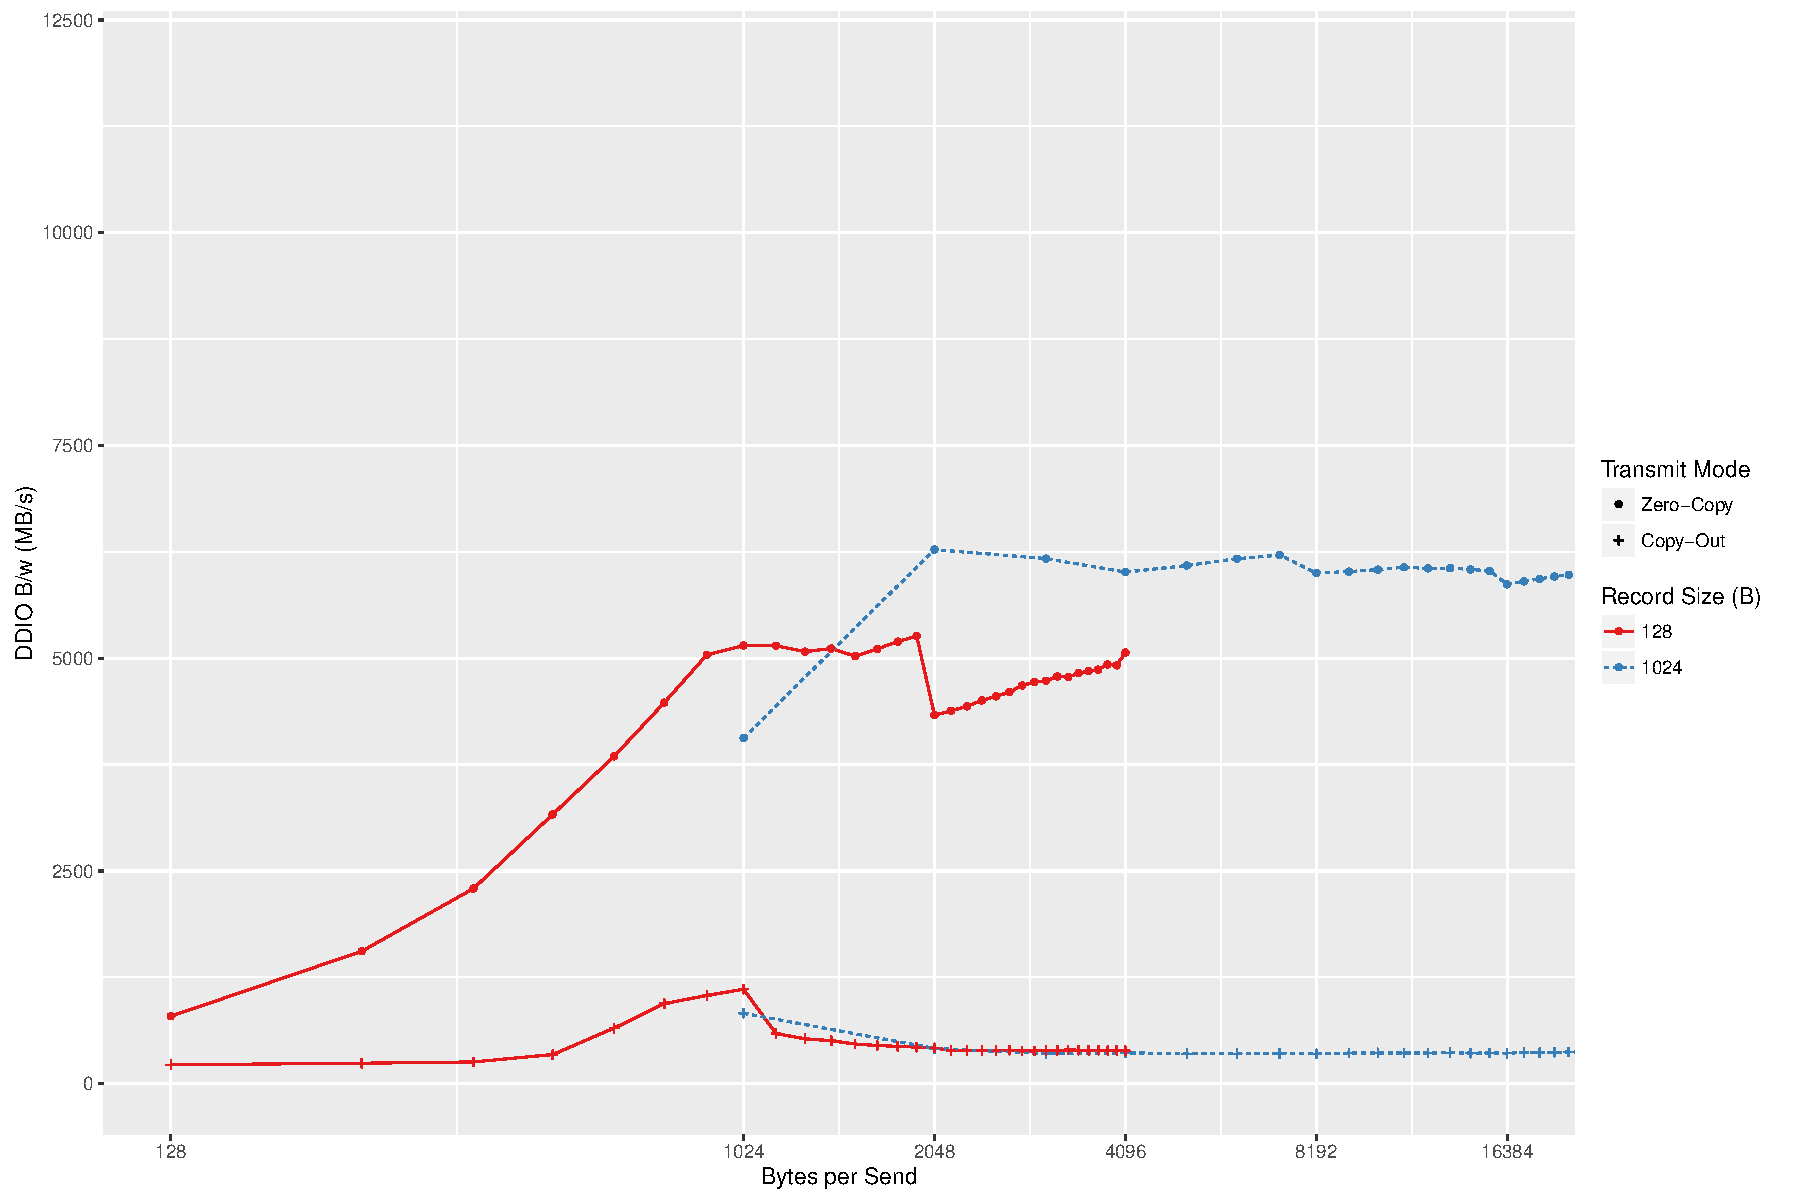
\includegraphics[width=\textwidth]{fig-ddiobw.pdf}
\caption{DRAM accesses (MB/s) LLC misses from DDIO vs Throughput}
\label{fig:ddiobw}
\end{figure}



\subsection{DDIO savings in Copy Out}
\label{sec:ddiobw-savings}
The previous sections showed how Copy Out can be costly and degrade system performance because of the consumed memory bandwidth. We also examined how DDIO traffic plays a big role 
in modern CPU architecture in limiting I/O costs. We are going to examine the interesting side effect of the additional \memcpy~ . Figure ~\ref{fig:ddiobw-percent} shows what percentage of consumed 
memory bandwidth results from misses from the DDIO region. It tells us that While we pay the price of \memcpy to bring data to the LLC, it actually helps in limiting further DRAM access while transmitting 
from the region reserved for DDIO. If not for this effect, both Copy Out and Zero Copy might have added Memory Bandwidth consumption in bringing data from DRAM for transmission. 
\begin{figure}[H]
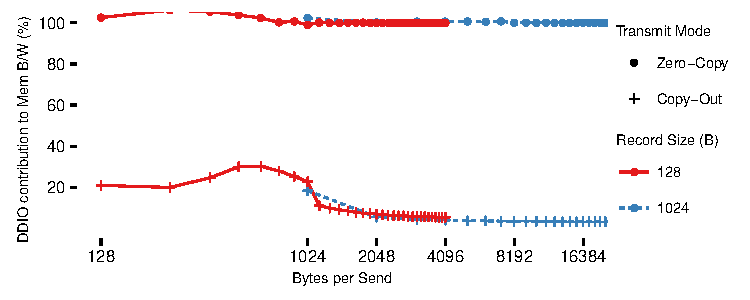
\includegraphics[width=\textwidth]{fig-ddiobw-percent.pdf}
\caption{Percentage of LLC misses that contribute to Total memory bandwidth consumed}
\label{fig:ddiobw-percent}
\end{figure}


\framebox[0.9\textwidth][c]{
  \parbox{0.7\textwidth}{
  \textbf{Takeaways: Copy Out side effects of DDIO}
  \begin{enumerate}
  \item The additional \memcpy ~ step pre-fetches data to LLC at a cost and improves the number of DDIO misses that result in DRAM accesses. 
  \item If not for the DDIO effects, we would have seen a bigger drop in throughput and memory efficiency for Copy Out. 
  \end{enumerate}
  \textbf{Recommendation}: DDIO paints a slightly different picture of memory consumption favoring Copy Out; In the bigger scheme of things, Total memory bandwidth consumed still makes us prefer Zero Copy \label{takeaway:impact-ddiobw-savings}
 }}


\section{Anomaly in Transmission Throughput}
\label{sec:anomaly}
While evaluating performance and efficiency of Zero Copy in previous sections, we saw that for 128~B records, the transmission throughput doesn't linearly progress 
on increasing the transmission size. If you refer back to Figure~\ref{fig:zero-copy-tput}, throughput trends upward until we reach 1024~B(8 records), the transmission throughput remains consistent for about 8-16 records and 
then the performance tapers off. There is a huge dip in transmission throughput going from 15 to 16 records and even though the performance gradually recovers, it doesn't quite 
catch up with Copy Out until we get to the maximum number of records possible and even at that point Copy Out edges Zero Copy performance by a bit. After some investigation, we discovered 
that LLC bytes read from memory due to misses due to PCIe jumps to the peak measured reads and then saturates and the anomaly corresponds to these data points. 

Figure~\ref{fig:pciebw} shows the read requests issued by LLC because of misses from PCIe traffic. For 128~B records, we can clearly see that after 8 records, this metric is 
nearly saturated and at 16 records, the number of bytes read peaks causing the dip in transmit performance. The memory reads due to PCIe traffic is saturated at this point and 
we can see a similar trend for 1024~B records too. Since larger records packs more data per record, the dip in transmit performance is not evident in that case. The other interesting 
thing to realise is that for Copy Out, the amount of memory traffic induced by PCIe errors follows a similar trend as transmission throughput which is expected since 
NIC itself is connected via PCIe interface.
\begin{figure}[t]
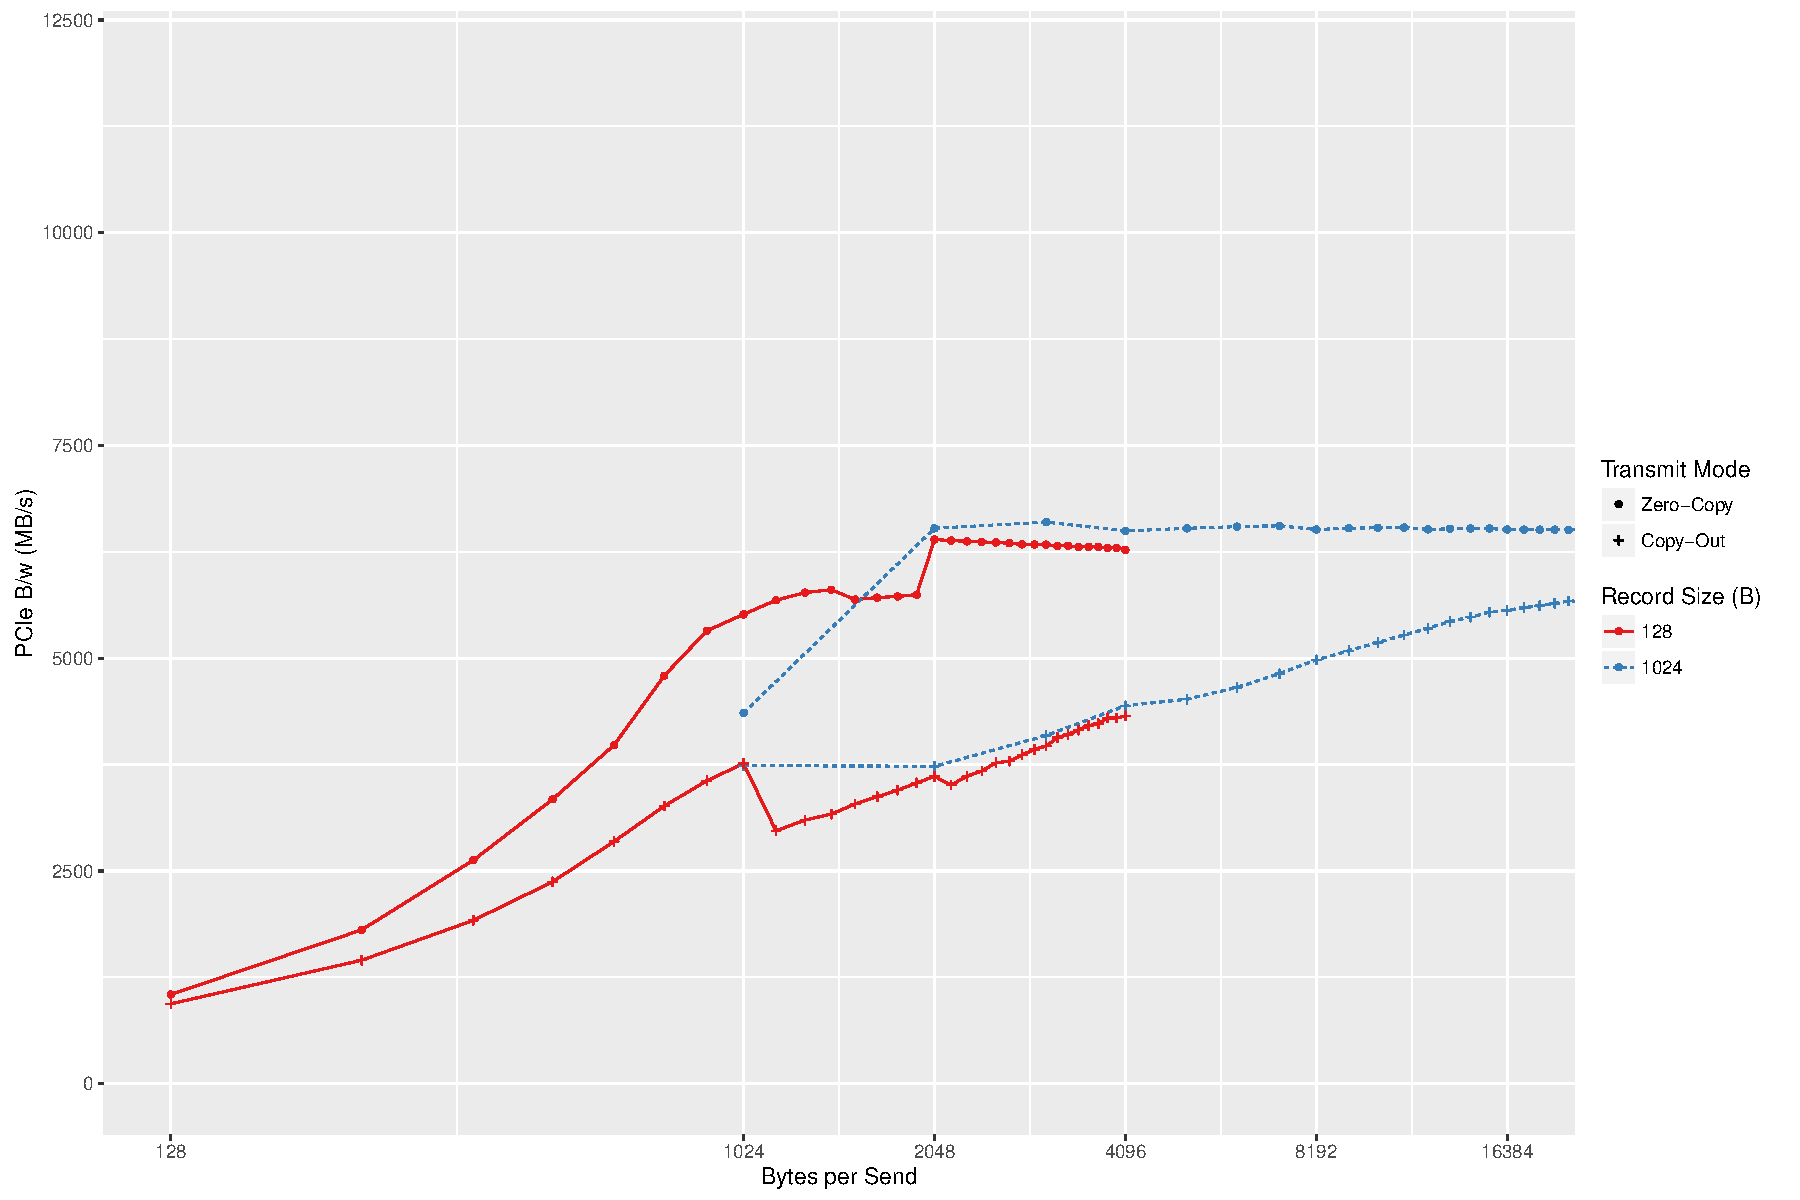
\includegraphics[width=\textwidth]{fig-pciebw.pdf}
\caption{DRAM accesses (MB/s) due to LLC misses due to PCIe}
\label{fig:pciebw}
\end{figure}


\subsection{PCIe induced DRAM accesses and Throughput}
Figure ~\ref{fig:pciebw-ratio} shows the ratio of DRAM accesses induced by PCIe traffic to the obtained transmission throughput for various data points. When we transmit 16 smal records (2048~B),
the PCIe effectiveness goes down and the ratio peaks. This is strictly in line with transmission throughput shown in Figure~\ref{fig:zero-copy-tput} where at 2048~B, we see a sharp drop in transmission 
throughput which it slowly recovers from as we increase the number of S/G entries per transmission. There is an inverse correlation between the ratio of PCIe induced DRAM accesses and Transmission throughput
\begin{figure}[t]
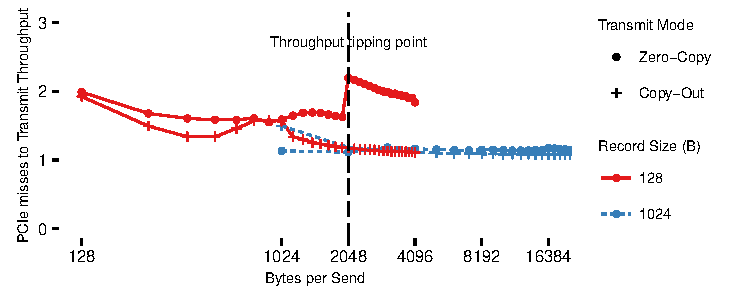
\includegraphics[width=\textwidth]{fig-pciebw-ratio.pdf}
\caption{Ratio of DRAM accesses because of PCIe to Transmission throughput}
\label{fig:pciebw-ratio}
\end{figure}



\framebox[0.9\textwidth][c]{
  \parbox{0.7\textwidth}{
  \textbf{Takeaways: DRAM accesses due to PCIe traffic and anomaly in Throughput}
  \begin{enumerate}
  \item The memory utilisation because of PCIe peaks as transmission througput drops for small records doing Zero Copy.
  \end{enumerate}
  \label{takeaway:impact-membw}
 }}


\section{Conclusions}
\begin{itemize}
\item For large sets of small records, Copy Out offers better performance; if your record sizes are larger, use Zero Copy
\item Zero Copying larger records will give you good memory bandwidth utilisation
\item DDIO compensates for some of the memory bandwidth cost to Copy Out data if transmissions are smaller; this is irrelevant in the bigger scheme of things.
\item Careful tuning of parameters is required if you were to only use Zero Copy; PCIe induced memory accesses maybe the reason Copy Out outperforms Zero Copy for certain parameters. 
\end{itemize}

